\documentclass{article}

% NeurIPS 2026 main track, anonymized double-blind submission.
% Switch to \usepackage[preprint]{neurips_2026} for an arXiv-style preprint
% with author names visible. Use [main, final]{neurips_2026} only after
% acceptance for the camera-ready.
\usepackage{neurips_2026}

\usepackage[utf8]{inputenc}
\usepackage[T1]{fontenc}
\usepackage{hyperref}
\usepackage{url}
\usepackage{booktabs}
\usepackage{amsfonts}
\usepackage{amssymb}
\usepackage{amsmath}
\usepackage{nicefrac}
\usepackage{microtype}
\usepackage{xcolor}
\usepackage{graphicx}
\usepackage{enumitem}

\title{Dynamic Disequilibrium:\\
       An Agent-Based Mechanism for Bubbles\\
       without Biased Agents}

\author{%
  Anonymous Author(s)\\
  Affiliation\\
  Address\\
  \texttt{email}\\
}

\begin{document}

\maketitle

\begin{abstract}
We present the \emph{Estimated Dynamic Equilibrium Model} (EDEM), an
agent-based framework in which supply and demand are realisations of
a coupled stochastic process driven by heterogeneous, error-prone
agent valuations. The framework's central technical contribution is
a generative mechanism for persistent disequilibrium: when
market-clearing prices are repeatedly selected from the upper tail of
noisy bid distributions and fed back into future valuations, expected
prices drift upward even with strictly zero-mean estimation errors.
We derive the bias in closed form for a clean special case
($\sigma(n-1)/(n+1)$ for $n$ iid uniform bids, which is the
classical winner's curse) and show via simulation that compounding
the bias across epochs produces exponential price growth without any
behavioural assumption about investor optimism. EDEM extends
\citet{miller1977}'s divergence-of-opinion theory to a fully dynamic
setting and recovers Walrasian equilibrium and Miller's static
premium as limiting cases. Eight controlled experiments in the
Python ABM framework Mesa, on a $32 \times 32$ real-estate
neighbourhood, plus a 30-cell sensitivity grid, demonstrate six
qualitatively distinct regimes---all reachable from the same agent
ruleset. The result has direct implications for machine-learning
valuation algorithms (Zestimate-style automated valuation models):
trained on historical clearing prices, such systems are by
construction fitting an upper-order statistic of plausible sale
prices rather than fair value, and at deployment time function as
positively-biased point estimators.
\end{abstract}

\section{Introduction}
\label{sec:intro}

The Efficient Market Hypothesis remains the dominant theory of price
formation. It predicts when prices reflect available information but
does not provide a generative microstructural account of when and
why they fail to: bubbles, crashes, persistent cross-sectional
return anomalies, and the stylised observation that real markets
very rarely sit at the textbook supply--demand fixed point. Decades
of empirical work have produced rival theories whose claims often
contradict one another, because abundant and noisy financial data
can be mined to support nearly any hypothesis \citep{moffitt2017}.

The central technical claim of this paper is that two structural
features---max-bid clearing and per-epoch feedback of clearing
prices into agent valuations---generate persistent positive drift in
realised market prices even when individual agents' estimation errors
are exactly zero-mean. The mechanism is order-statistic bias: each
seller selects the maximum of multiple noisy bids, and the maximum
of $n$ zero-mean draws is, in expectation, strictly above their
mean. Feeding the realised maximum back into the next round's anchor
compounds the bias multiplicatively. No behavioural assumption about
investor optimism, risk aversion, or attention is required.

This is a dynamic generalisation of the classical winner's curse
\citep{thaler1988winners}: the same upper-tail-selection effect that
biases the expected payment in a single common-value auction, fed
epoch-to-epoch into the next anchor value, produces unbounded
drift in market valuations.

The implication for machine-learning valuation matters for the
NeurIPS audience. An ML valuation algorithm trained on historical
clearing prices---automated valuation models (AVMs), iBuying
pricing models, comparable-sale algorithms---is not fitting fair
value. By construction it is fitting the upper-order statistic of
plausible sale prices, because the clearing price is the maximum of
the bids received. At deployment time it functions as a
positively-biased point estimator that may itself provide the market
with a coordinating signal pulling realised winning bids further
upward.

\paragraph{Contributions.}
\begin{enumerate}[leftmargin=*,nosep]
\item An order-statistic mechanism for bubbles without biased
agents (Section~\ref{sec:mechanism}): in closed form, for a clean
special case, the expected winning bid exceeds the home value by
$\sigma(n-1)/(n+1)$ when $n$ bidders draw zero-mean errors with
dispersion $\sigma$. Compounded across epochs this produces
exponential price drift.
\item A unified framework (Section~\ref{sec:framework}) that nests
Walrasian equilibrium and Miller's static premium as limiting
cases, and admits a family of out-of-equilibrium regimes (business
cycles, persistent overshoots and undershoots, runaway bubbles,
constant transition) parameterised by estimation noise, balancer
strength, and time-on-market.
\item Eight controlled experiments plus a 30-cell sensitivity
grid (Section~\ref{sec:experiments}) demonstrating that the
order-statistic drift produces price drift above textbook
equilibrium in $100\%$ of parameter combinations tested.
\item A discussion of implications for ML valuation systems
(Section~\ref{sec:discussion}) connecting the model to
selection-aware estimation procedures that AVM deployers should
adopt.
\end{enumerate}

\section{Background and Related Work}
\label{sec:background}

\citet{miller1977} proposed a static model in which the $N$ shares
of a stock are sold to the $N$ most optimistic of $K > N$ potential
investors, so the clearing price reflects the marginal optimist
rather than the mean valuation. Greater divergence of opinion thus
produces a price \emph{premium}, and (because future returns are
earned against the elevated price) lower subsequent returns. The
half-century of empirical literature that grew up around this claim
has not converged: the \emph{discount} camp argues divergence of
opinion proxies for risk and predicts higher future returns
\citep{williams1977,mayshar1983,varian1985,merton1987,epsteinwang1994},
while the \emph{premium} camp finds the opposite
\citep{doukas2006}. \citet{moffitt2017} summarises the impasse.

The static framing is the source of the empirical confusion.
Miller's model specifies a one-shot relationship between beliefs
and the market-clearing price. Real markets are continuous
processes in which today's price feeds into tomorrow's beliefs.
We show that the same upper-tail-selection mechanism that produces
Miller's premium (and, separately, the winner's curse
\citep{thaler1988winners} in common-value auctions) generates a
\emph{dynamic} drift when iterated---and that the same underlying
mechanism can produce either a premium or a discount in finite
samples, which explains why empirical work has found both.

Closely related work in agent-based economics has used ABMs to
study housing markets \citep{baptista2016boe,geanakoplos2012leverage}
and behavioural finance generally \citep{shiller2003}. The
contribution here is the structural identification of the
selection mechanism, formalised analytically and validated
empirically across a parameter sweep.

\section{The EDEM Framework}
\label{sec:framework}

A market is staged on a finite torus $G$ of homes, with $Q_s(t)$
sellers $\mathcal{S}_t$ (one per home, immobile) and $Q_d(t)$ buyers
$\mathcal{B}_t$ (mobile, walking the torus). Each home $h$ has a fixed
unobservable fair value $v^{*}(h)$ and a market value $v_t(h)$ that
evolves. Each agent $i$ valuing home $h$ at tick $t$ draws an
estimation
\begin{equation}
\label{eq:estimation}
E_{i,t}(h) = v_{t}(h)\,(1+\varepsilon_{i,t,h}),
\qquad
\varepsilon_{i,t,h} \stackrel{\mathrm{iid}}{\sim} F_{i}(\sigma_{i}),
\end{equation}
with $\mathbb{E}[\varepsilon] = 0$. The three-way index is essential:
each \emph{bid} is an independent draw. Throughout, $\sigma_i$ is
expressed as a decimal ($0.05$ means $\pm 5\%$ maximum error);
parameter tables report percentages.

A buyer that lands on a seller's home posts a bid
$\beta_{b,s}^{(t)} = E_{b,t}(h(s))$. Sellers accumulate bids; on
patience timeout, the seller offers to sign with the buyer holding
the best bid. The buyer commits iff
\begin{equation}
\label{eq:cond2}
\beta \;\ge\; \frac{1}{|\mathcal{B}_b|}\sum_{\beta'\in\mathcal{B}_b}\beta',
\end{equation}
where $\mathcal{B}_b$ is the buyer's outstanding bid set (including
$\beta$). Eq.~\eqref{eq:cond2} is order-statistic selection on the
buyer's side: committing only when the offered bid is at or above
the buyer's running benchmark restricts purchases to the upper tail
of the buyer's own bid distribution.

The realised market price is the output of a clearing functional
$p_t = A(X_t;\theta)$ over the full market state $X_t$. We study
two instantiations. In the discrete-event \emph{DE} variant, $A$ is
the rolling average of the last $W$ completed sales:
\begin{equation}
\label{eq:price-rolling}
p_{t} = \frac{1}{m_{t}}\sum_{j=k(t)-m_{t}+1}^{k(t)} P^{\mathrm{sale}}_{j},
\qquad m_{t} = \min(W, k(t)),
\end{equation}
where $k(t)$ counts completed sales up to tick $t$. In the
speculative \emph{EDEM} variant there are no realised sales; instead
each home's value updates multiplicatively at the end of every
epoch of $T$ ticks:
\begin{equation}
\label{eq:value-update}
v_{t+T}(h) = v_t(h)\cdot \bar r_t,
\quad
\bar r_t = \frac{1}{|\mathcal{Y}_t|}\sum_{b\in\mathcal{Y}_t}\min_{s\in\mathcal{W}_b(t)}\frac{\beta_{b,s}^{(t)}}{v_t(h(s))}
\end{equation}
when the set $\mathcal{Y}_t$ of buyers holding at least one winning
bid is non-empty (else $\bar r_t = 1$). $\mathcal{W}_b(t)$ is the
set of sellers on which buyer $b$ holds the winning bid.

The supply and demand quantities are themselves integer-valued
random walks driven by the price increment
$\Delta p_{t-1} = p_{t-1} - p_{t-2}$:
\begin{equation}
\label{eq:balancer}
Q_{s}(t) = Q_{s}(t-1) + Z^{s}_{t},
\quad
\mathbb{E}[Z^{s}_{t}] = C_{b}\,\mathrm{sgn}(\Delta p_{t-1}).
\end{equation}
With $C_{b} > 0$ rising prices add sellers (mean-reverting); with
$C_{b} < 0$ rising prices remove sellers (trend-following); with
$C_{b} = 0$ the population is frozen. A symmetric equation governs
$Q_d$. A population floor of one agent per side truncates the random
walk in extreme regimes.

Setting $\sigma_i \equiv 0$ collapses Eq.~\eqref{eq:estimation} to
universal agreement; the order-statistic drift vanishes and EDEM
approaches the Walrasian fixed-point equilibrium. Retaining
$\sigma_i > 0$ but freezing the dynamics ($T \to \infty$, single
period, no value update) recovers a Miller-style static premium
mechanism.

\section{The Order-Statistic Mechanism}
\label{sec:mechanism}

\paragraph{Closed-form bias.}
Consider a seller $s$ receiving $n \ge 2$ bids $\beta_i = v_t(h(s))(1+\varepsilon_i)$ with $\varepsilon_i \sim \mathcal{U}[-\sigma, +\sigma]$ iid. The expected winning bid is
\begin{equation}
\label{eq:ostat-bias}
\mathbb{E}\!\left[\frac{\max_i \beta_i}{v_t(h(s))}\right]
= 1 + \mathbb{E}\!\left[\max_i \varepsilon_i\right]
= 1 + \sigma\,\frac{n-1}{n+1},
\end{equation}
using the order-statistic identity for the maximum of $n$ iid
uniform variates. The right-hand side strictly exceeds 1 for all
$n \ge 2$ and $\sigma > 0$; the gap grows in both $n$ and $\sigma$.

\paragraph{Relation to the winner's curse.}
Eq.~\eqref{eq:ostat-bias} also recovers the classical winner's curse
as a static special case. In a common-value auction, the winning
bidder is selected precisely because her signal is the most
favourable draw among the bidder pool. The curse is thus an
order-statistic selection effect before it is a behavioural
failure: optimism is not required for the winning bid to be
upward-selected. Rational bid shading can correct the expected
payment in a static auction, but it does not remove the allocation
fact that the winning signal comes from the upper tail. EDEM's
contribution is to feed that upper-tail clearing price into the
next period's valuation anchor, turning the one-period
winner's-curse effect into a dynamic drift mechanism.

\paragraph{What Eq.~\eqref{eq:ostat-bias} does and does not prove.}
Eq.~\eqref{eq:ostat-bias} establishes that the seller-side maximum
has expected ratio strictly above 1. The per-epoch update
Eq.~\eqref{eq:value-update} compounds a related but distinct
quantity $\bar r_t$ (the buyer-side mean of $\min_s$ winning
ratios), for which we have no closed form. Two further care points
apply when moving from the theorem to sample-path behaviour:
\emph{(i)} for an iid multiplicative process $v_T = v_0\prod_t r_t$,
the expectation $\mathbb{E}[v_T] = v_0\,(\mathbb{E}[r])^T$ grows
multiplicatively whenever $\mathbb{E}[r]>1$, but the median is
governed by $\mathbb{E}[\log r]$; by Jensen's inequality
$\mathbb{E}[r]>1$ does not on its own imply
$\mathbb{E}[\log r]>0$. \emph{(ii)} The fallback $\bar r_t = 1$ for
empty-winner epochs puts a point mass at unity that the clean
theorem does not capture.

\paragraph{Empirical bridge.}
Table~\ref{tab:rbar} reports the distribution of $\bar r_t$
extracted directly from our EDEM-regime simulations, with
$\bar r_t = v_{t+T}(h)/v_t(h)$ at every epoch boundary across all
seeds. The growth condition $\mathbb{E}[\log \bar r_t] > 0$ holds
in every regime, certifying sample-path exponential growth and
closing the gap between Eq.~\eqref{eq:ostat-bias} and the simulated
buyer-min update.

\begin{table}[h]
\centering
\caption{Empirical distribution of $\bar r_t$ across $1500$ epochs
per regime (10 seeds, 150 epochs/seed). The growth condition
$\mathbb{E}[\log \bar r_t] > 0$ holds in every regime examined.}
\label{tab:rbar}
\small
\begin{tabular}{l c c c c}
\toprule
\textbf{Regime} & $\mathbb{E}[\bar r_t]$ & $\Pr(\bar r_t>1)$ & $\mathbb{E}[\log \bar r_t]$ & median$\,\bar r_t$ \\
\midrule
Run 6 ($C_b=0$, $\bar\sigma=0.15$)        & 1.0429 & 83.5\% & $+0.0411$ & 1.044 \\
Run 7 ($C_b=+1$, $\bar\sigma=0.15$)       & 1.0104 & 19.7\% & $+0.0098$ & 1.000 \\
Run 7 ($C_b=-1$, $\bar\sigma=0.15$)       & 1.0153 & 25.4\% & $+0.0144$ & 1.000 \\
Run 8 ($C_b=-1$, $\bar\sigma$ growing)    & 1.0287 & 24.9\% & $+0.0236$ & 1.000 \\
\bottomrule
\end{tabular}
\end{table}

\section{Implementation}
\label{sec:implementation}

EDEM is implemented in the Python ABM framework Mesa
\citep{masad2015mesa} on a $32 \times 32$ toroidal
$\mathtt{MultiGrid}$, matching the wrapped patch world of the
original NetLogo prototypes from which this work descends. Per-cell
state ($v_t(h)$, $v^*(h)$, last sale price, last sale tick) is a
lightweight dataclass attached to each grid cell; buyers and sellers
are $\mathtt{mesa.Agent}$ subclasses. Bids are mirrored
dictionaries on each side. The rolling 25-sale market price of
Eq.~\eqref{eq:price-rolling} is a $\mathtt{deque(maxlen=25)}$. The
per-epoch update in Eq.~\eqref{eq:value-update} fires on a
cycle-counter trick one tick before buyers reset, preserving their
winning-bid flags. The balancer Eq.~\eqref{eq:balancer} fires
$\lfloor |C_b| \rfloor$ deterministic swaps per epoch plus one
Bernoulli swap with probability $|C_b| - \lfloor |C_b| \rfloor$;
sign of $C_b$ controls direction. A population floor of one agent
per side prevents the balancer from killing the last agent.

The Mesa model and 42 pytest unit tests fit in under 600 lines
including docstrings. Each experiment script seeds the model
deterministically and runs 10 seeds. Total reproduction time on a
2024-era laptop is approximately 25 minutes (CPU only). Code and
data are released under MIT licence at a URL provided in the
camera-ready version of this paper.

\section{Experiments and Results}
\label{sec:experiments}

Eight controlled experiments grouped into two regimes (DE: Runs 1--5,
discrete-event sales; speculative-market EDEM: Runs 6--8,
multiplicative value updates) plus a 30-cell sensitivity grid
(Run 9). Each experiment runs 10 seeds; figures plot the median
across seeds with the 10th--90th percentile band. Full parameter
tables are in Appendix~\ref{app:params}; per-run figures for runs
not shown inline here are in Appendix~\ref{app:allfigs}.

\paragraph{The six regimes.} Table~\ref{tab:regimes} consolidates
the end-of-run statistics. The eight runs sweep three parameter
axes (estimation noise $\bar\sigma$, seller patience, balancer
$C_b$) and produce six qualitatively distinct steady-state
regimes---band-stable, business-cycle, persistent overshoot,
persistent undershoot, runaway bubble, and constant transition---
all reachable from the same agent ruleset.

\begin{table}[h]
\centering
\caption{Eight EDEM runs: parameters and observed outcomes
(median across $\ge 8$ seeds). DE runs report median deviation of
the rolling market price from the textbook equilibrium; EDEM runs
report $v_t/v^*$.}
\label{tab:regimes}
\small
\begin{tabular}{l l l l}
\toprule
\textbf{Run} & \textbf{Manipulated parameter} & \textbf{Outcome metric} & \textbf{Regime} \\
\midrule
1 & $\bar\sigma=0.05$, patience $\le 50$       & $-2\%$ to $+11\%$ band      & band-stable        \\
2 & $\bar\sigma=0.25$                          & $-17\%$ to $+34\%$ periodic & business-cycle     \\
3 & patience $\le 100$                         & $+14\%$ persistent          & overshoot          \\
4 & demand intercept $-50$                     & $-18\%$ persistent          & undershoot         \\
5 & shock at $t=3000$, then re-shocks          & moving-target chase         & transitional       \\
\midrule
6 & EDEM, $C_b = 0$, $\bar\sigma=0.15$         & $v_t/v^* = 421\times$       & runaway bubble     \\
7 & EDEM, $C_b\in\{-1, 0, +1\}$                & $7.7, 421, 4.2\times$ resp. & balancer-shaped    \\
8 & EDEM, $C_b=-1$, $\bar\sigma$ growing       & $v_t/v^* = 30\times$        & super-linear       \\
\bottomrule
\end{tabular}
\end{table}

\paragraph{Bubble regime under no balancer.}
With balancer disabled ($C_b = 0$) and $\bar\sigma = 0.15$, the
market exhibits a clean log-linear bubble (Fig.~\ref{fig:bubble}):
the median value-to-true ratio multiplies $\sim 421\times$ over
3000 ticks, with a tight band. The mechanism is exactly that of
Section~\ref{sec:mechanism}: each epoch's average winning ratio
$\bar r_t$ is $>1$ in expectation, and Eq.~\eqref{eq:value-update}
compounds it multiplicatively.

\begin{figure}[h]
\centering
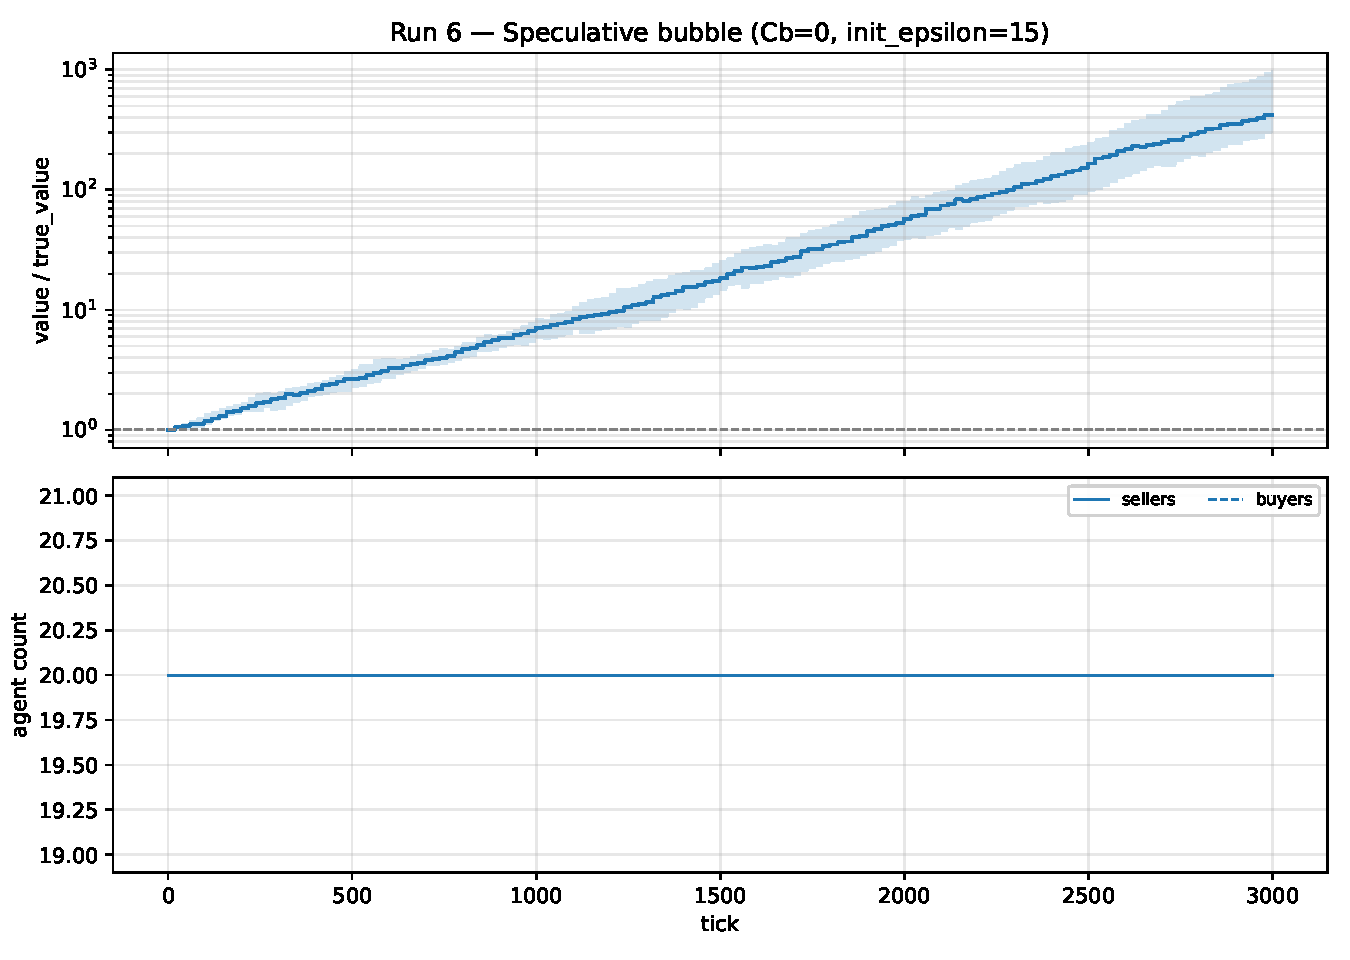
\includegraphics[width=0.85\linewidth]{figures/fig6_bubble}
\caption{Run 6 (bubble, $C_b=0$, $\bar\sigma=0.15$). Top: median
$v_t/v^*$ (log scale) with $10$--$90$ percentile band. Bottom:
agent counts (frozen at $20$ each because $C_b=0$).}
\label{fig:bubble}
\end{figure}

\paragraph{Balancer-coefficient sweep.}
Varying $C_b \in \{+1, 0, -1\}$ at fixed $\bar\sigma = 0.15$ yields
three qualitatively distinct trajectories (Fig.~\ref{fig:balancer}):
the mean-reverting case ($C_b=+1$) plateaus near $4\times$ as the
population drifts toward sellers; the trend-following case
($C_b=-1$) reaches $\sim 7.7\times$ with the population drifting
toward buyers; the no-balancer case dominates both at $\sim 421\times$.
This refines a prior claim in the literature that trend-following
should be the most explosive regime: in the Mesa simulation, the
trend-following balancer drains sellers to a single agent, leaving
fewer total sellers to inflate; the no-balancer case maintains
balanced populations and admits all of the upward bid-selection
bias unfiltered. No setting of $C_b$ in this grid restores
$v_t/v^* = 1$.

\begin{figure}[h]
\centering
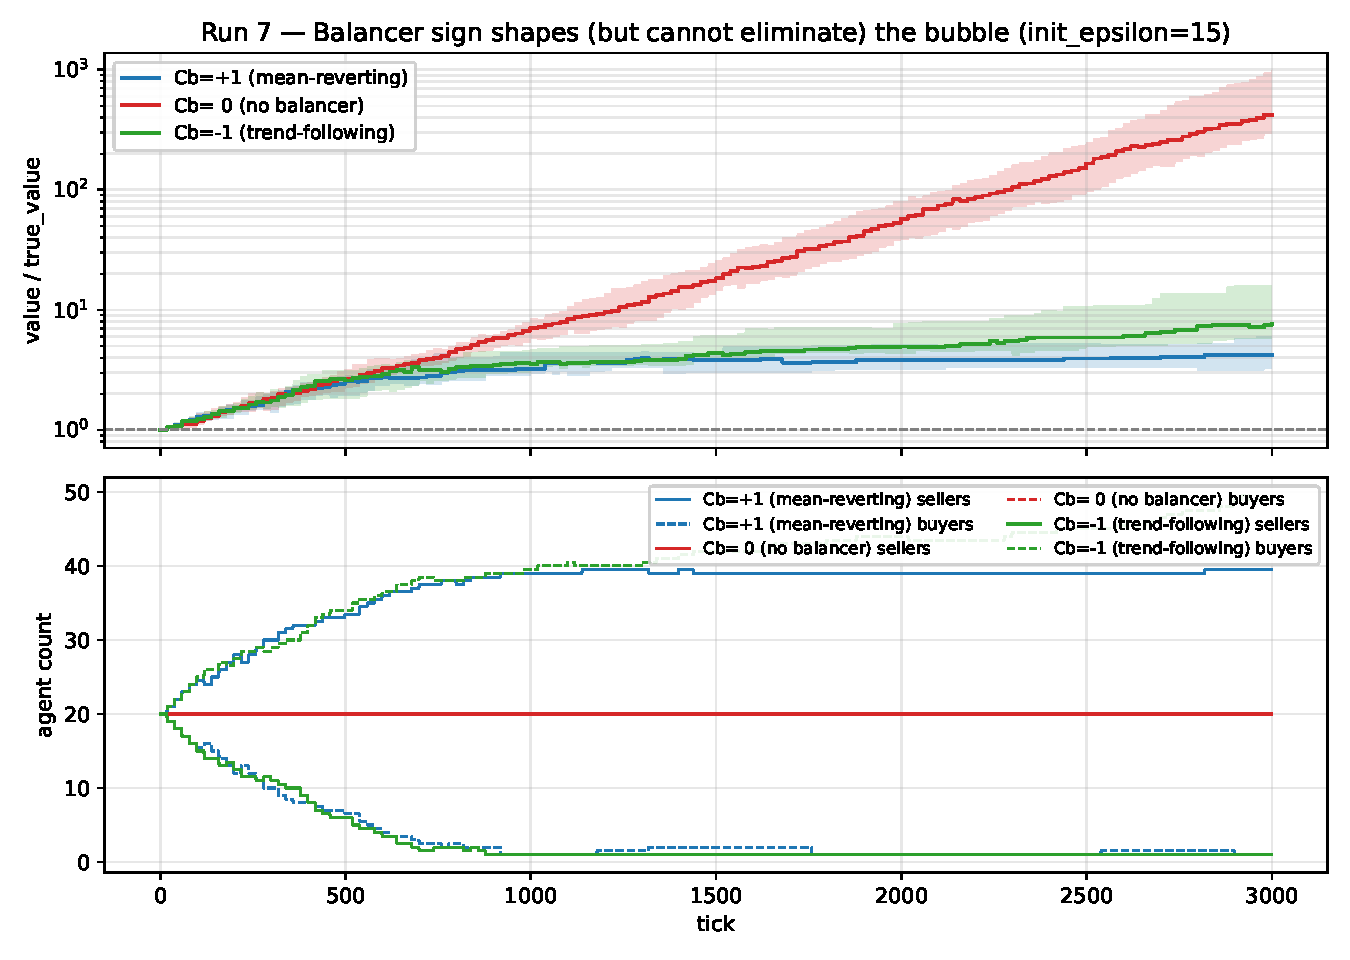
\includegraphics[width=0.85\linewidth]{figures/fig7_balancer_sweep}
\caption{Run 7 (balancer sweep at $\bar\sigma=0.15$). The three
regimes are overlaid; $C_b=0$ produces the strongest bubble. The
population panel shows the one-vs-many state the strong balancers
induce.}
\label{fig:balancer}
\end{figure}

\paragraph{Sensitivity to $C_b$ and $\bar\sigma$.}
A $5\times 6$ grid sweeps $C_b \in \{-1, -0.5, 0, +0.5, +1\}$ and
$\bar\sigma \in \{0.05, 0.10, 0.15, 0.20, 0.25, 0.30\}$, with 5
seeds per cell at 1500 ticks (Fig.~\ref{fig:sensitivity}). Every
cell of the grid has $v_t/v^* > 1$, and $43\%$ of cells exceed
$10\times$ within $1500$ ticks. The order-statistic drift is
universal across the parameter grid, not a corner case. $C_b = 0$
dominates within every $\bar\sigma$ column.

\begin{figure}[h]
\centering
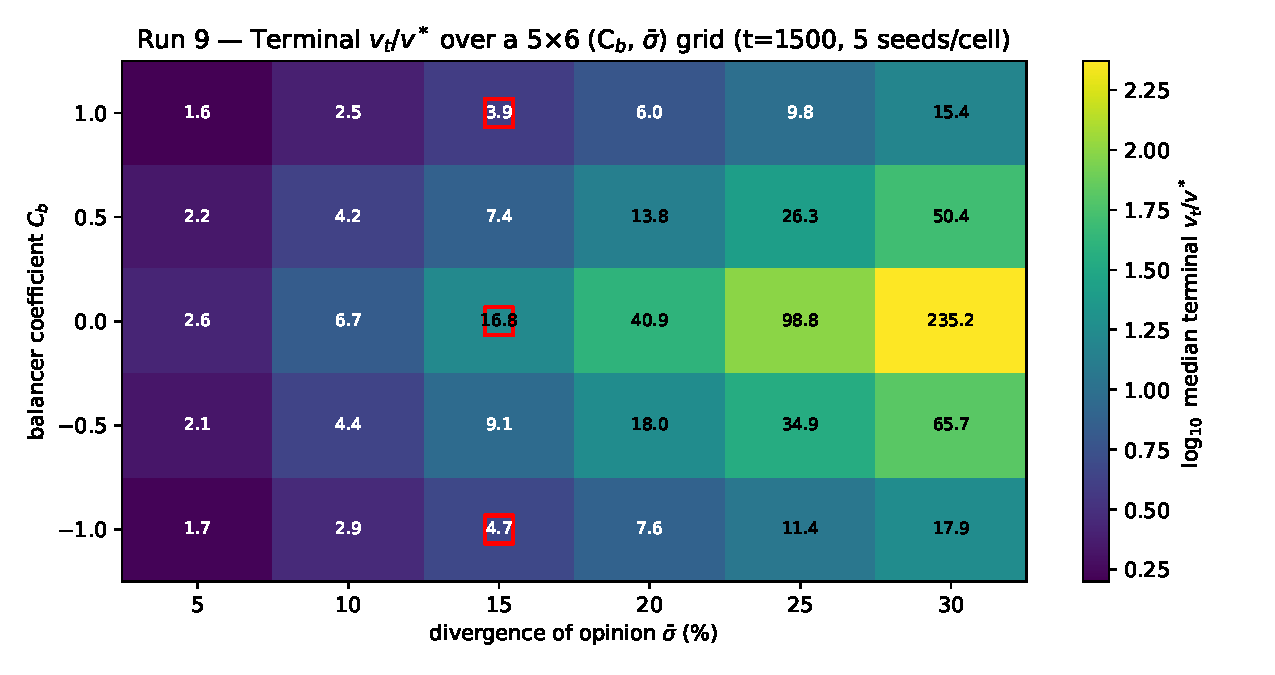
\includegraphics[width=0.95\linewidth]{figures/fig9_sensitivity}
\caption{Run 9 (sensitivity heatmap). Median terminal $v_t/v^*$
over a $5\times 6$ ($C_b$, $\bar\sigma$) grid, log colour scale.
Red squares mark cells corresponding to Runs 6 and 7. Every cell
exceeds 1.0; 43\% exceed 10.0.}
\label{fig:sensitivity}
\end{figure}

\paragraph{Other regimes.} DE Runs 1--5 produce the band-stable,
business-cycle, overshoot, undershoot, and transitional regimes
listed in Table~\ref{tab:regimes}. Run 4 (low agent density): mean
realised price $p \approx 41$ versus textbook $p^* = 50$, an
$18\%$ shortfall, with episodes reaching $p \approx 37$ ($26\%$ at
the trough). Run 5 (shocked market): the realised price never
settles when demand is toggled every $2000$ ticks. The figures for
these runs are in Appendix~\ref{app:allfigs}.

\section{Discussion: Implications for ML Valuation}
\label{sec:discussion}

\paragraph{Bid-selection asymmetry, not estimation bias, drives bubbles.}
The estimation function Eq.~\eqref{eq:estimation} has zero mean
error: an agent's expected valuation is exactly the home's current
value. Yet the EDEM speculative regime produces unbounded upward
drift even with this unbiased estimator. The mechanism is not
behavioural bias but a statistical asymmetry: each seller selects
the maximum bid received, and the maximum of $N$ noisy estimates
of a fair value is, in expectation, larger than the fair value
itself. Eq.~\eqref{eq:value-update} compounds this asymmetry
multiplicatively across epochs. This is the dynamic generalisation
of the classical winner's curse \citep{thaler1988winners}.

\paragraph{Implication for ML valuation systems.}
The same mechanism operates in any pricing system whose inputs are
anchored to recent market-clearing prices. A machine-learning
valuation algorithm trained on historical sale prices is, by
construction, fitting the upper-order statistic of plausible sale
prices for a similar asset---the maximum of the relevant noisy
estimates---not their mean. Deployed at scale, such an algorithm
functions as a positively-biased point estimator that may provide
the market with a coordinating signal pulling realised winning
bids further upward, feeding back into the next training cycle.

A defensible deployment would correct for this: predict the
median rather than the mean of plausible sale prices; use a
censored-data likelihood that accounts for the offer-acceptance
threshold; or use an explicitly rank-aware estimator that targets
fair value rather than winning-bid value. The 2021 wind-down of
Zillow's algorithmic-iBuying programme \citep{zillow2021ibuying}
is one episode in which a clearing-price-anchored valuation system
at scale incurred substantial losses; we do not advance EDEM as a
complete account of that specific event, but the public record is
consistent with the mechanism here.

\paragraph{Why empirical premium/discount studies disagree.}
Each empirical sample of the divergence-of-opinion premium is a
finite-window observation along a coupled stochastic process
governed by $\sigma$ and $C_b$. Two studies sampling distinct
positions on distinct trajectories may both correctly observe
opposite signs. The unifying claim from EDEM is not that one camp
is right and the other wrong, but that the static framing has been
asking the wrong question; the relevant quantity is the trajectory
of $\bar r_t$, not its sign at a snapshot.

\section{Limitations and Conclusion}
\label{sec:conclusion}

EDEM models a single asset class with no leverage, no macroeconomic
environment, and non-adaptive (non-learning) agents. The
30-cell sensitivity grid covers a defensible range of $(C_b, \bar\sigma)$
but does not explore extreme $|C_b|$ values where the population
dynamics qualitatively change. Run 5's shock-recovery scenario uses
a 12{,}000-tick budget that is too short for the market to reach
its post-shock floor before the patience boost fires. Bayesian-belief
and reinforcement-learning extensions of the agent rule set
(Appendix~\ref{app:extensions}) are sketched but not implemented.

The contribution we believe travels beyond the EDEM setting is the
mechanism. Bubbles, persistent disequilibrium, and the empirical
contradictions in the divergence-of-opinion literature do not
require behavioural bias to explain. Repeated upper-tail selection,
fed back into subsequent valuations, is sufficient. For the
NeurIPS audience the practical consequence is concrete: an ML
valuation model trained on historical clearing prices is by
construction fitting an upper-order statistic, and selection-aware
estimation is a deployment-time requirement, not an academic
nicety.

\bibliographystyle{plainnat}
\bibliography{references}

\clearpage
\appendix

\section{ODD Protocol}
\label{app:odd}

This appendix documents EDEM in the standard ODD protocol for
agent-based models \citep{grimm2020odd}.

\paragraph{Purpose and patterns.} EDEM characterises the conditions
under which an agent-based real-estate market reaches a stable
equilibrium price, and identifies the mechanisms that prevent
equilibrium when they do not. Patterns the model reproduces: stable
band-bounded equilibria; endogenous business cycles; persistent
shifts in the realised price relative to the textbook equilibrium
under altered patience or density; multiplicative price drift in
the absence of a balancer.

\paragraph{Entities, state variables, scales.}
Entities: Buyers and Sellers ($\mathtt{mesa.Agent}$ subclasses),
Homes (per-cell dataclass on a $32\times 32$ toroidal grid).
Buyer state: epsilon (estimation-error bound), delay, current bid,
heading; EDEM variant adds the lowest-bid-to-value ratio and a
yellow (winning) flag. Seller state: epsilon, patience timer,
current ask price, dictionary of received bids; EDEM adds number of
bids, total bids, best-bid-to-value, best-bid-to-true-value. Home
state: market price, last-sale tick, last-sale price, fair value
$v^{*}$, current value $v$. Model state: rolling window of last 25
sale prices (DE), epoch counter (EDEM), cross-population epsilon
(EDEM). One spatial unit = one home; one tick is the smallest
temporal unit. DE balance period is 100 ticks; EDEM epoch is 20.

\paragraph{Process overview.}
Per tick: (i) each agent steps once, in randomised order over both
classes; a Buyer's step posts bids, then wiggles, then steps
forward; a Seller's step processes patience and best-bid logic;
(ii) the model invokes the balancer (DE: every 100 ticks; EDEM:
every 20 ticks via the cycle-counter trick that preserves
buyers' winning-bid flags); (iii) the data collector samples
model-level reporters.

\paragraph{Design concepts.}
\emph{Basic principles}: EDEM extends the divergence-of-opinion
premise of \citet{miller1977} to a multi-period setting; agents
act on noisy estimates of an unobservable fair value.
\emph{Emergence}: the price level, agent population dynamics, and
macroscopic regimes emerge from local interaction; none of these
phenomena are coded in directly.
\emph{Adaptation}: sellers lower ask prices when patience elapses
without high-enough bids (the only adaptive behaviour). Buyers do
not adapt.
\emph{Objectives}: sellers maximise realised sale price subject to
patience. Buyers commit only to offers whose realised bid is at or
above their own running benchmark (Eq.~\eqref{eq:cond2})---a
selection rule, not a price-minimisation objective.
\emph{Learning, prediction}: none in the baseline model.
\emph{Sensing}: buyers sense whether a seller is on their patch;
sellers sense the bids in their own bid table; neither senses the
global market price directly.
\emph{Interaction}: direct via mirrored-dictionary updates; indirect
via the average ask price and rolling sale-price average influencing
newly-spawned agents.
\emph{Stochasticity}: agent placement, buyer heading, epsilon draws,
per-bid error draws, victim selection, Bernoulli draws for
fractional $C_b$ swaps---all from a single seeded
$\mathtt{numpy.random.Generator}$.
\emph{Observation}: per-tick model reporters stacked into Parquet
datasets, one per seed.

\paragraph{Initialisation.}
DE: spawn $\mathtt{equi\_qnty}$ sellers at random unique cells
with patience $\sim \mathcal{U}[0, \mathtt{init\_patience})$ and
ask price drawn from $\mathcal{U}[-\bar\sigma, +\bar\sigma]$
around $p^*$; spawn $\mathtt{equi\_qnty}$ buyers at random cells.
EDEM: 20 sellers and 20 buyers, all homes initialised with
$v_0(h) = v^*(h) = 100$.

\paragraph{Input data and submodels.}
No external input data; EDEM is closed. Estimation function:
Eq.~\eqref{eq:estimation}. Bid acceptance: Eq.~\eqref{eq:cond2}.
Market price: Eq.~\eqref{eq:price-rolling} (DE) and
Eq.~\eqref{eq:value-update} (EDEM). Balancer: Eq.~\eqref{eq:balancer}
in finite-population form with population floor of one.

\section{Parameter Tables}
\label{app:params}

\paragraph{Common parameters across all runs.}
World size $32\times 32$ toroidal; seeds per run $\ge 8$ (typically
10); bid-acceptance rule \texttt{netlogo} (the rule actually coded
in the original 2018 NetLogo source, matching Eq.~\eqref{eq:cond2}).

\paragraph{DE runs 1--5.}
Supply $\hat Q_s(p) = a_s + 0.5\,p$, $a_s = 0$. Demand
$\hat Q_d(p) = a_d - 0.5\,p$, $a_d = 100$ (Runs 1--3, 5) or $50$
(Run 4) or $\{125, 75\}$ alternating (Run 5 Scenario B). Maximum
valuation error $\bar\sigma$: $0.05$ (Runs 1, 3--5) or $0.25$
(Run 2). Maximum patience: $50$ (Runs 1, 2, 4) or $100$ (Run 3)
or $50 \to 165$ at $t=7000$ (Run 5 Scenario A). Balance period
$T_B = 100$. Sale window $W = 25$. Ticks per seed: $20{,}000$
(Runs 1--4), $12{,}000$ (Run 5).

\paragraph{EDEM runs 6--8.}
Initial $\bar\sigma$: $0.15$ (Runs 6, 7) or $0.05$ (Run 8).
$\bar\sigma$ growth per epoch: $0$ (Runs 6, 7) or $+0.005$ (Run 8).
Balancer $C_b$: $0$ (Run 6); $\{+1, 0, -1\}$ (Run 7); $-1$ (Run 8).
Initial buyers / sellers: $20/20$. Epoch length 20 ticks. Ticks per
seed: 3000. True value $v^*(h) = 100$ uniform across all homes.

\paragraph{Run 9 sensitivity grid.}
$C_b \in \{-1, -0.5, 0, +0.5, +1\}$; $\bar\sigma \in \{0.05, 0.10,
0.15, 0.20, 0.25, 0.30\}$. 5 seeds per cell, 1500 ticks each.

\section{All Experiment Figures}
\label{app:allfigs}

\begin{figure}[h]
\centering
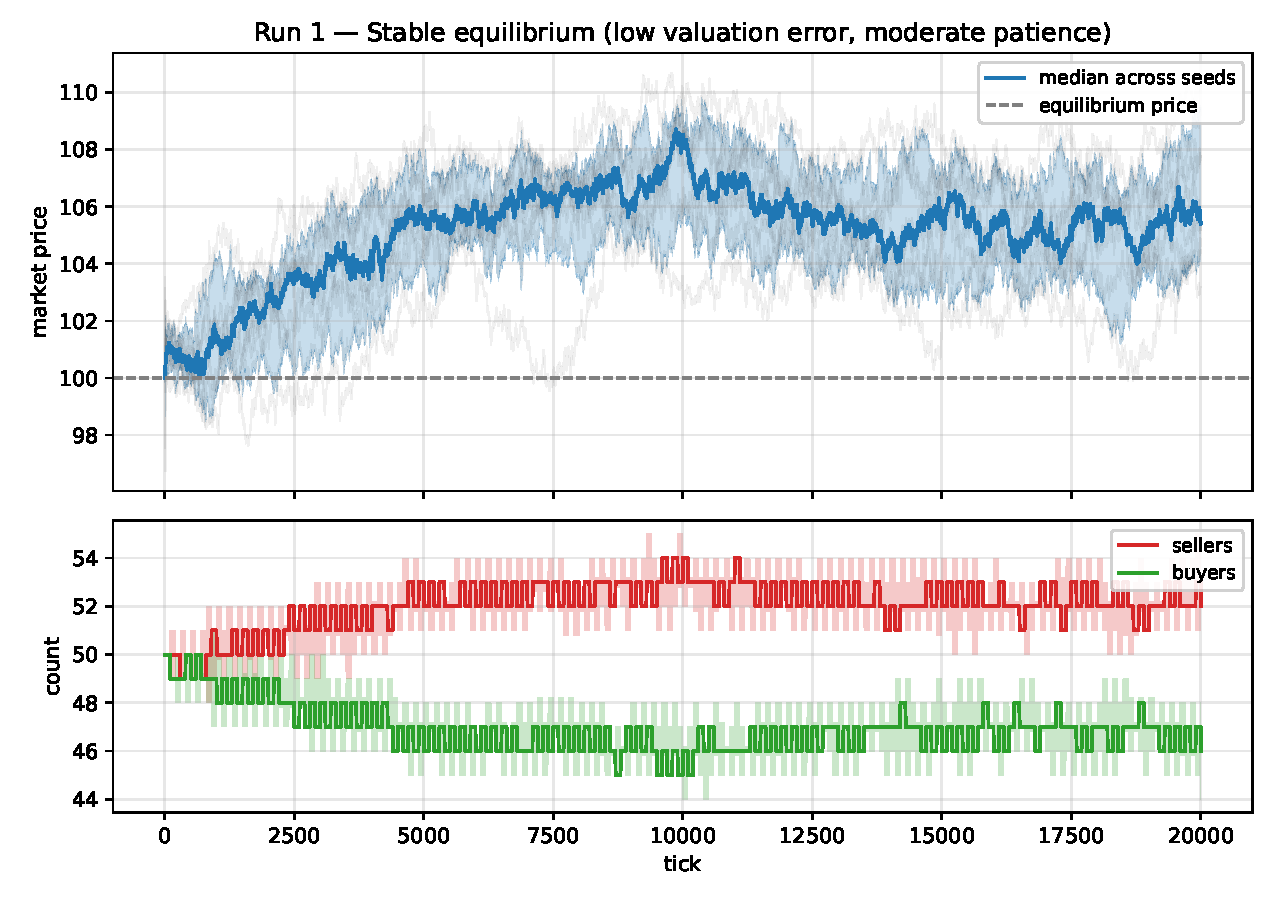
\includegraphics[width=0.85\linewidth]{figures/fig1_stable}
\caption{Run 1 -- Stable equilibrium with low valuation error and
moderate patience.}
\label{fig:run1}
\end{figure}

\begin{figure}[h]
\centering
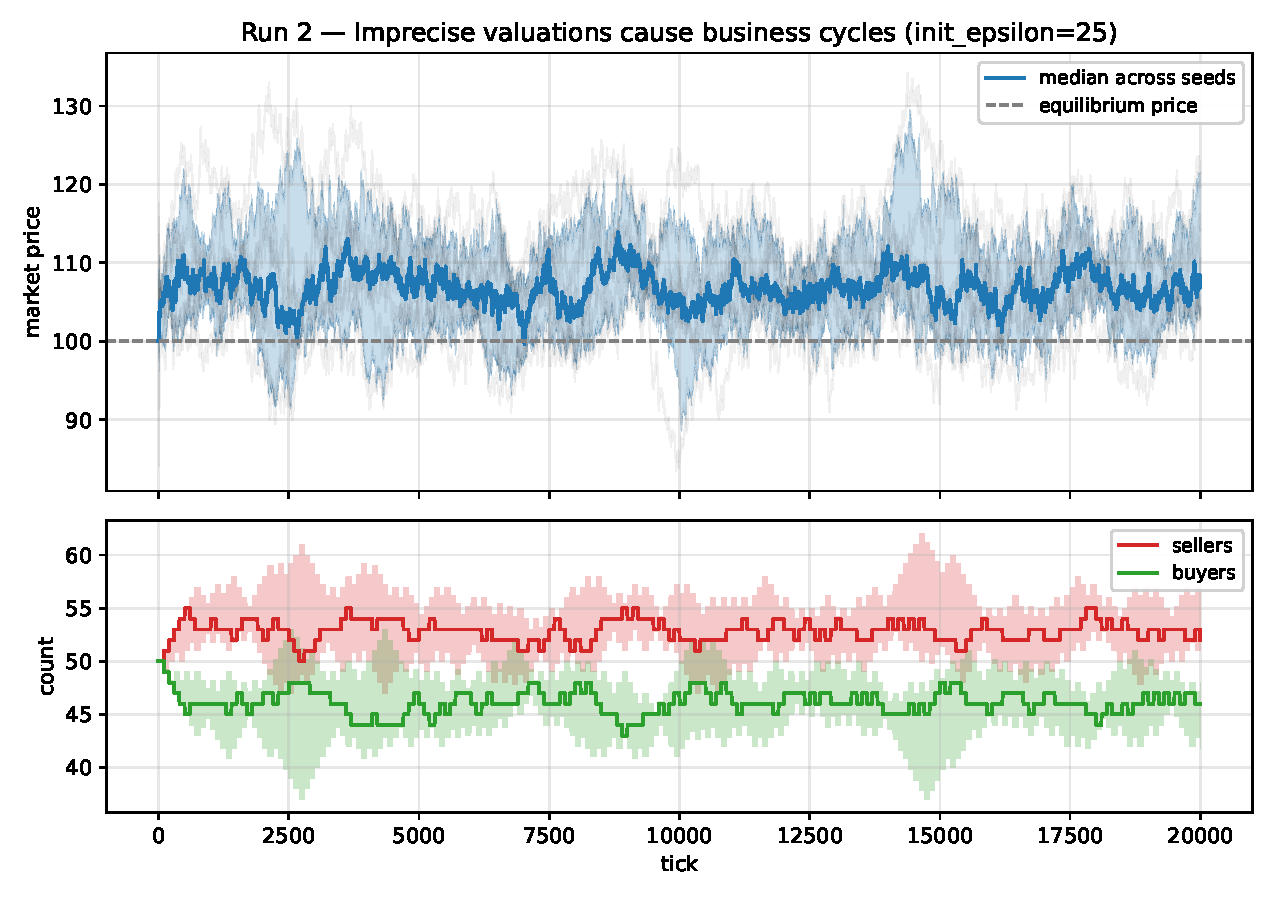
\includegraphics[width=0.85\linewidth]{figures/fig2_high_error}
\caption{Run 2 -- High valuation error ($\bar\sigma=0.25$) generates
endogenous business cycles.}
\label{fig:run2}
\end{figure}

\begin{figure}[h]
\centering
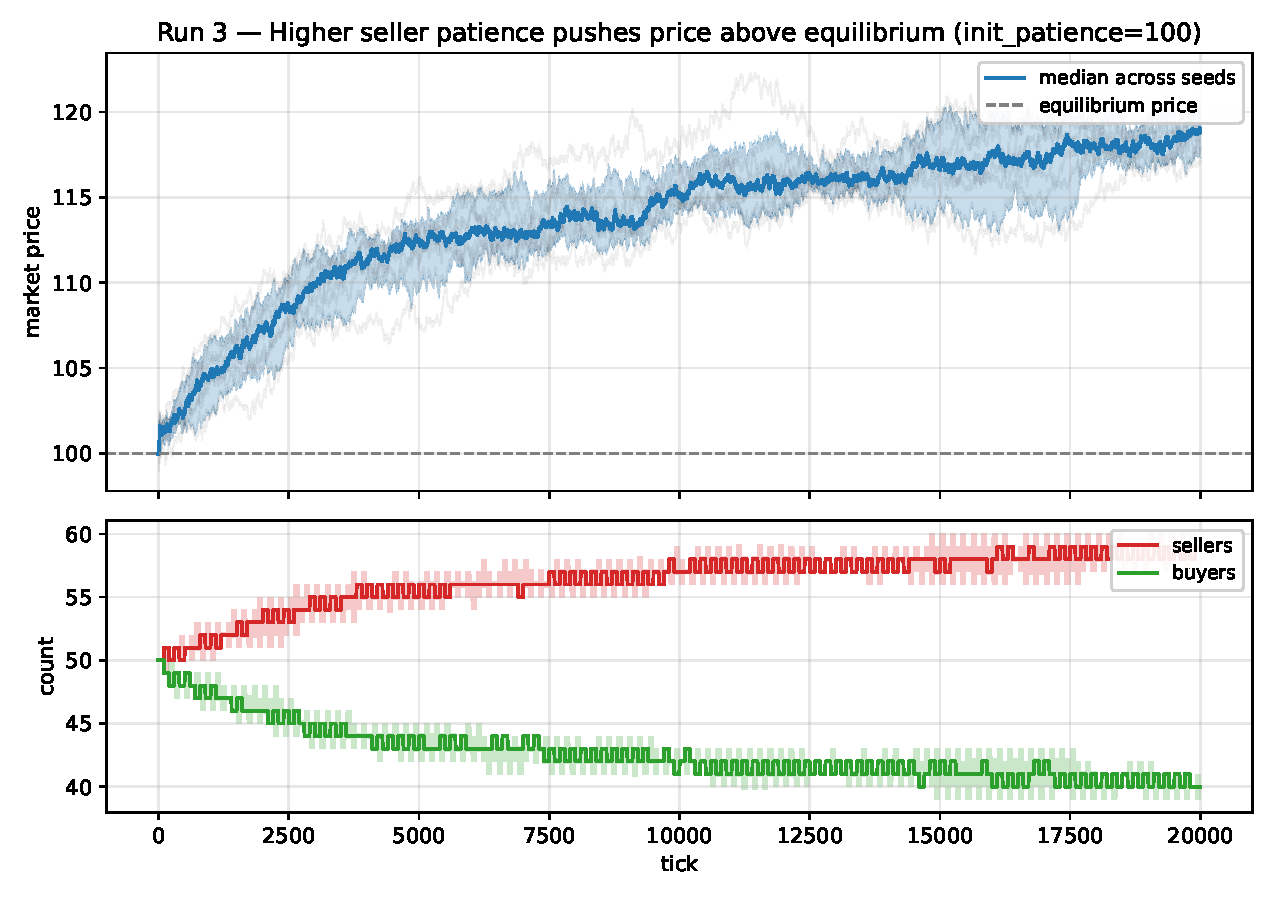
\includegraphics[width=0.85\linewidth]{figures/fig3_patience}
\caption{Run 3 -- Doubling seller patience to $100$ pushes the
market price about $14\%$ above the textbook equilibrium and
sustains it there.}
\label{fig:run3}
\end{figure}

\begin{figure}[h]
\centering
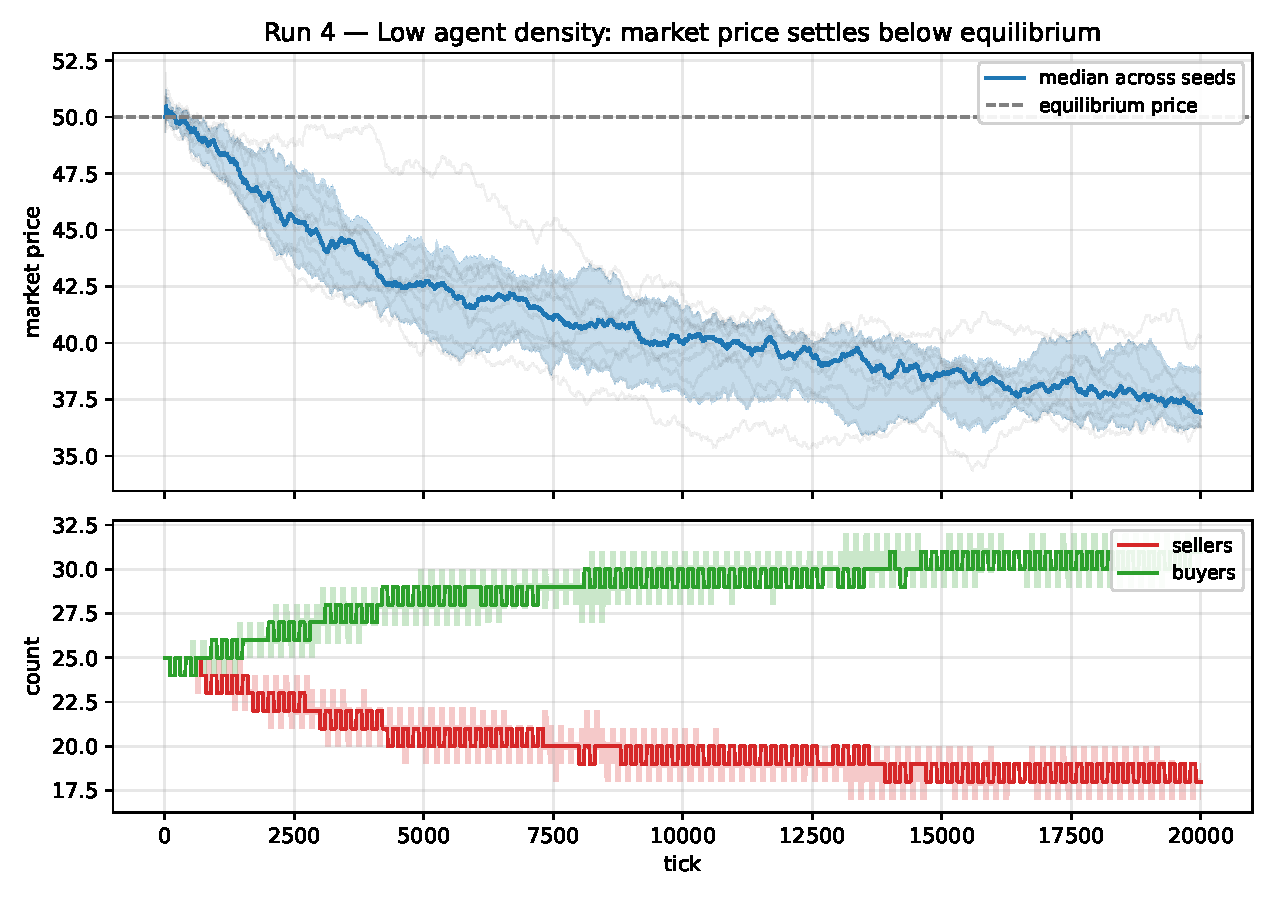
\includegraphics[width=0.85\linewidth]{figures/fig4_low_density}
\caption{Run 4 -- Halving the demand intercept reduces equilibrium
quantity to $25$; the realised market price settles about $18\%$
below the textbook equilibrium.}
\label{fig:run4}
\end{figure}

\begin{figure}[h]
\centering
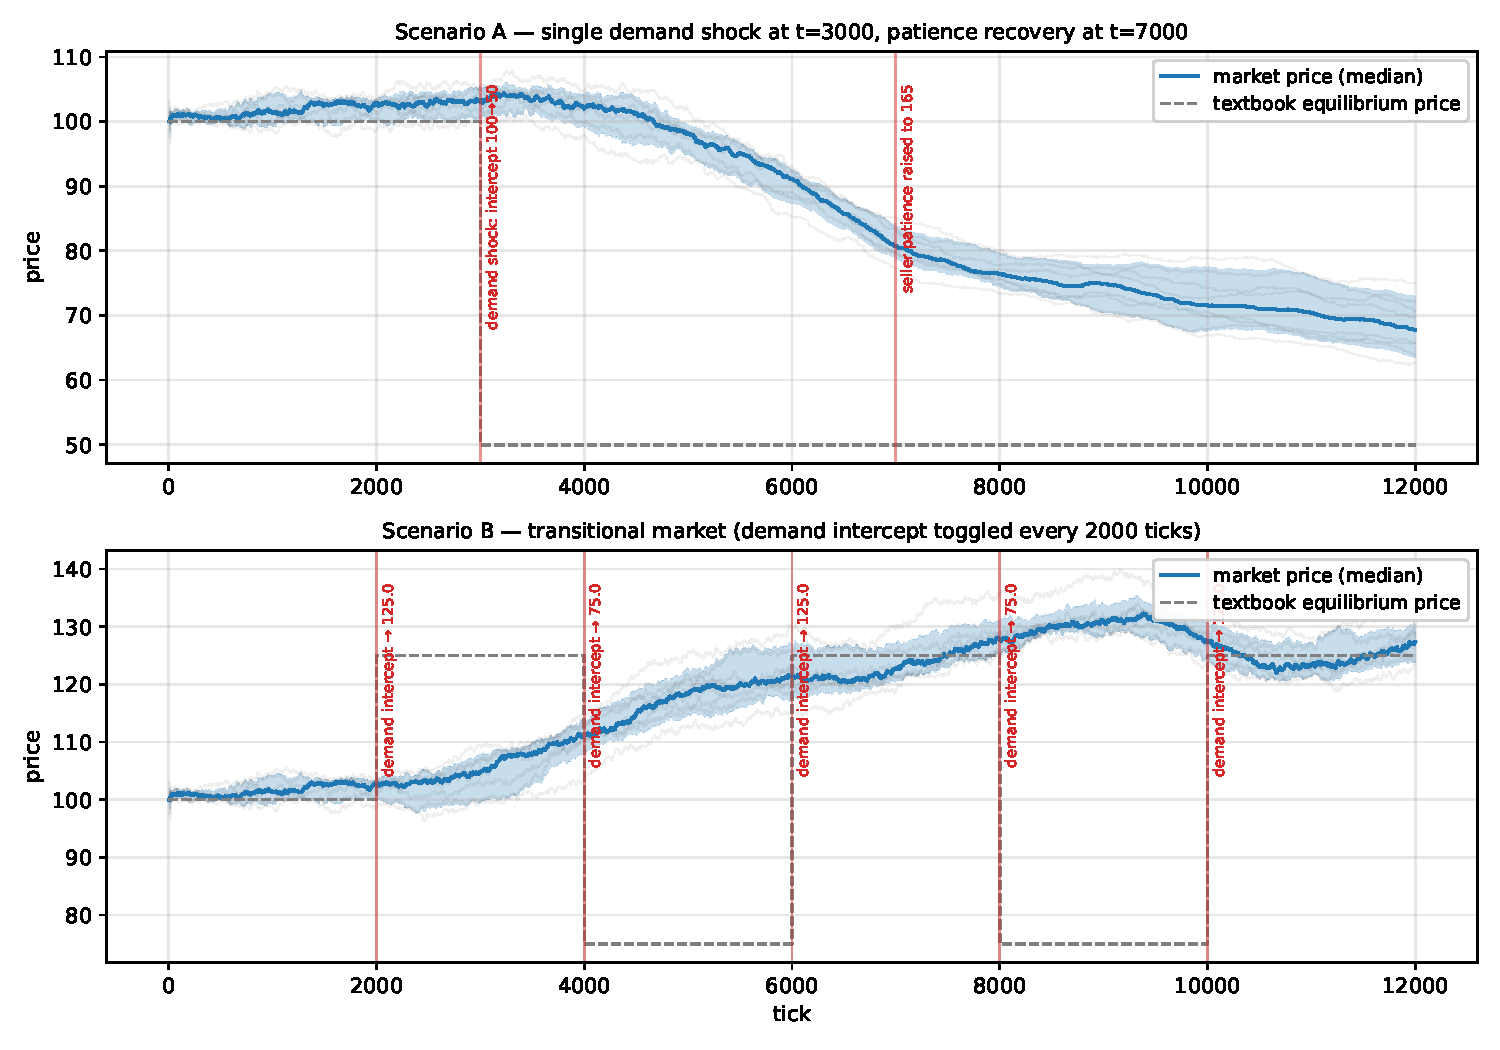
\includegraphics[width=0.9\linewidth]{figures/fig5_shock}
\caption{Run 5 -- Two shock scenarios. Top: a single demand shock
at $t = 3000$ followed by a patience boost at $t = 7000$. Bottom:
a transitional market in which demand toggles every $2000$ ticks.}
\label{fig:run5}
\end{figure}

\begin{figure}[h]
\centering
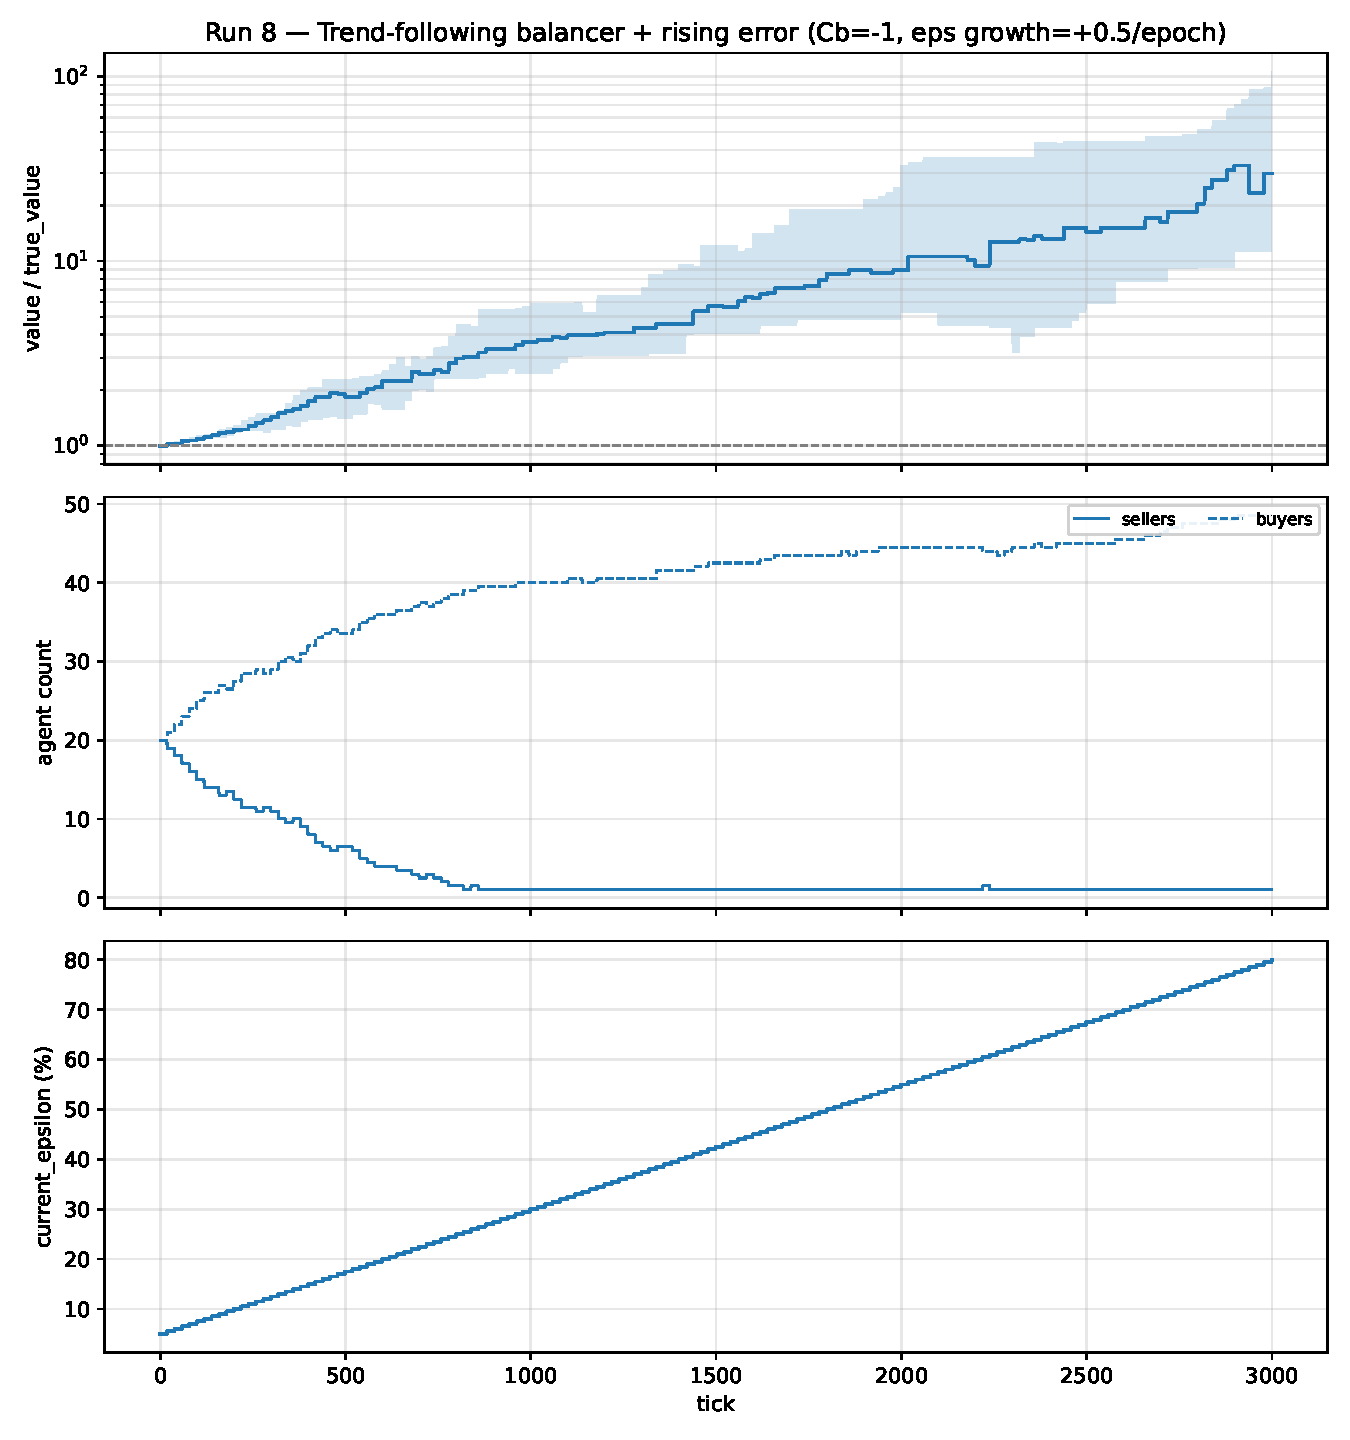
\includegraphics[width=0.85\linewidth]{figures/fig8_double_exp}
\caption{Run 8 -- Trend-following balancer ($C_b=-1$) combined
with linearly-growing $\bar\sigma$ ($0.05 \to 0.80$). The trajectory
is sustained super-linear rather than visibly double-exponential.}
\label{fig:run8}
\end{figure}

\section{Extensions and Future Work}
\label{app:extensions}

The framework of Section~\ref{sec:framework} is deliberately minimal
so that extensions can be plugged in without rewriting the agent
skeleton. Five directions are especially fruitful and we sketch
each below.

\paragraph{Bias-corrected clearing.} The bid-selection asymmetry
embedded in the max-bid clearing rule cannot be cancelled by any
linear balancer within the explored grid. Two replacements for the
clearing functional $A$ in Eq.~\eqref{eq:price-rolling} would
address it directly: (i) a winsorised mean replacing $\bar r_t$ in
Eq.~\eqref{eq:value-update}; (ii) a selection-aware estimator
substituting the median or lower-percentile of all bids
(not only winning bids) for $\bar r_t$. Either is a one-line edit
to the reference implementation.

\paragraph{Realtors and commission structures.} The DE seller is a
strict utility-maximiser whose only friction is patience. Real-world
residential transactions are intermediated by realtors whose payoff
is a fraction of the sale price. A realtor extension would replace
the seller agent with an aggregated listing agent whose patience
and ask-price strategies optimise expected commission across a
portfolio. This is a natural setting for empirical calibration:
realtor commission rates and listing durations are publicly
observable, unlike the patience parameter of the bare DE seller.

\paragraph{Open vs.\ blind auctions.} EDEM as posed is a blind-bid
model. Open-bid auctions substantially change the bid distribution
by exposing buyers to one another's valuations and would likely
amplify the bid-selection asymmetry.

\paragraph{Construction and the supply side.} A construction-market
variant inverts EDEM's agent roles: contractors bid downward to
win projects, with the lowest-bid contractor winning. The selection
asymmetry then operates in reverse, biasing realised contract
prices below the population fair value.

\paragraph{Adaptive agents.} EDEM agents are non-learning. A
Bayesian extension where each agent maintains a posterior over
fair value and updates after every observed sale would converge,
in the limit, toward bias-corrected estimation. A
reinforcement-learning variant with a buy-low/sell-high reward
would discover and exploit the bid-selection asymmetry; this would
be a computational analogue to the Zillow-Offers iBuying problem
\citep{zillow2021ibuying} and would offer a stress test of any
proposed clearing-rule fix.

\input{checklist.tex}

\end{document}
